\documentclass{beamer}
\usepackage[utf8]{inputenc}
\usepackage[spanish]{babel}
\graphicspath{ {/data/Documentos/Universidad/Fisymat2018/TFM/shh-signal-model/images/} }
\usepackage{graphicx,hyperref,ru,url}
\usepackage{color}
% The title of the presentation:
%  - first a short version which is visible at the bottom of each slide;
%  - second the full title shown on the title slide;
\title[Sonic Hedgehog signaling system]{
  Nuevo modelo para el sistema de señalización de Sonic Hedgehog}

% Optional: a subtitle to be dispalyed on the title slide
\subtitle{}

% The author(s) of the presentation:
%  - again first a short version to be displayed at the bottom;
%  - next the full list of authors, which may include contact information;
\author[Bartolomé Ortiz Viso]{
  Bartolomé Ortiz Viso \\\medskip
  {\small Tutor: Óscar Sánchez} }

% The institute:
%  - to start the name of the university as displayed on the top of each slide
%    this can be adjusted such that you can also create a Dutch version
%  - next the institute information as displayed on the title slide
\institute[Universidad de Granada]{
  Trabajo Fin de Máster  \\
  Máster en Física y Matemáticas}

% Add a date and possibly the name of the event to the slides
%  - again first a short version to be shown at the bottom of each slide
%  - second the full date and event name for the title slide
\date[14 Septiembre, 2018]{
  14 Septiembre, 2018}

\begin{document}

\begin{frame}
  \titlepage
\end{frame}

\begin{frame}
  \frametitle{Índice}
  \tableofcontents
\end{frame}

\section{Introducción}

\subsection{Motivación Biológica}
\begin{frame}
  \frametitle{Motivación Biológica}
\begin{center}
	Regulación génica y factores de transcripción
	
	\begin{figure}[h]
		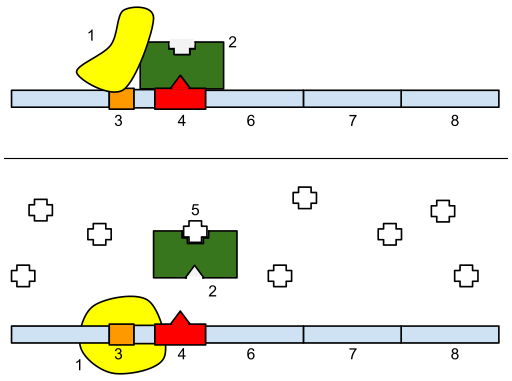
\includegraphics[width=0.5\textwidth]{fotobio2}
		\centering
		\caption{\small{1: ARN polimerasa, 2: represor, 3: promotor, 4: operador, 5: inhibidor del represor, 6-8: Genes}}
	\end{figure} 
\end{center}
\end{frame}

\subsection{Modelado BEWARE}
\begin{frame}
\frametitle{Calves del modelado BEWARE}
\begin{columns}
	\begin{column}{0.5\textwidth}
		{Objetivo:}
		
		\textbf{Extraer información sobre la regulación génica} a partir de las \textbf{secuencias de las regiones reguladoras} y la unión medida o inferida de los\textbf{ factores de transcripción específicos}.
		
	\end{column}
	\begin{column}{0.5\textwidth}
		 {Pasos comunes:}
		
		\begin{enumerate}
			
			\item  Se enumeran todos los estados posibles del potenciador y se calcula un peso estadístico asignado a cada estado.
			\item Asignamos un nivel de expresión génica de cada estado.
		\end{enumerate}
	\end{column}
\end{columns}


\end{frame}

\subsection{Definición del problema}

\begin{frame}
\frametitle{Problema a estudiar}
\textbf{Variables:} Gli y Ptc (a modelar por BEWARE), $Gli_3$ (FT activador), Gli3R (FT represor).
\begin{columns}
	\begin{column}{0.5\textwidth}
\begin{figure}
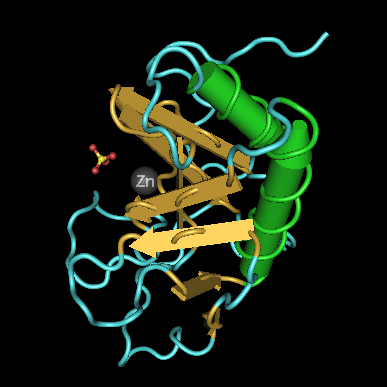
\includegraphics[width=0.8\textwidth]{shh_protein}\caption{Proteína Shh}
\end{figure}
\end{column}
\begin{column}{0.5\textwidth}
\begin{figure}
	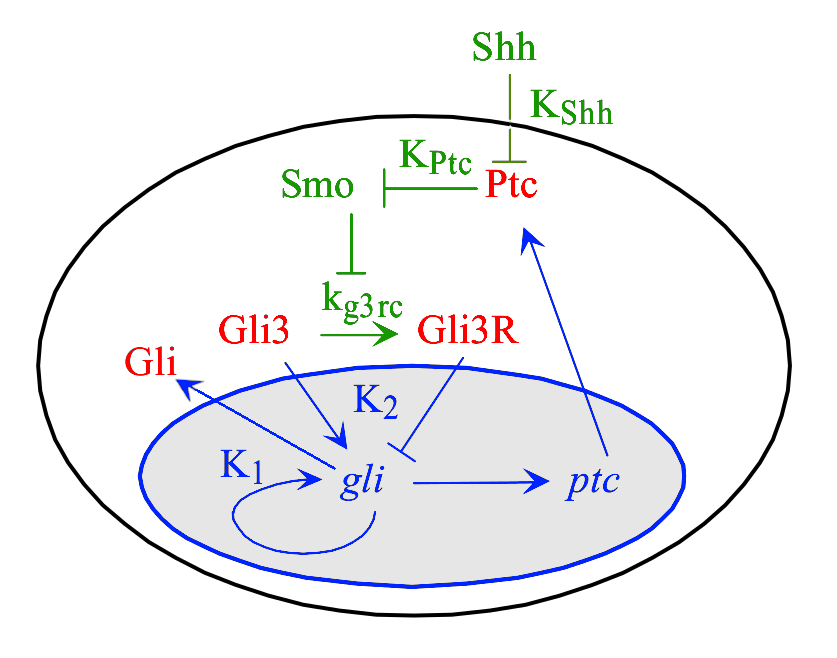
\includegraphics[width=1\textwidth]{signal_path_colors}\caption{descripción del sistema}
\end{figure}
\end{column}
\end{columns}
\end{frame}

\section{Modelo Lai-Saha}
\subsection{Definición del modelo}
\begin{frame}
  \frametitle{Modelo Lai-Saha (2004)}
\begin{columns}
	\begin{column}{0.5\textwidth}
		Claves:
		\begin{itemize}
			\item Proteólisis de $Gli_3$ según señalización de Shh y activación de la red. 
		\end{itemize}
			Claves \color{blue}BEWARE:
	\begin{itemize}
		\item Enfoque \textit{stimulated}.
		\item Expresión génica proporcional a la suma de factores de transcripción.
	\end{itemize}
	\end{column}
	\begin{column}{0.5\textwidth}
		{\tiny\[ \frac{dGli}{dt} = \color{blue}v_{max,G}Promoter+r_{bas,G}Basal\color{black}-k_{deg}Gli \]}
		{\tiny\[ \frac{dGli_3}{dt} = \frac{r_{g3b}}{Ptc}-Gli_3k_{deg}-Gli_3\left(\frac{k_{g3rc}}{K_{g3rc}+Signal}\right), \]}
		{\tiny\[ \frac{dGli3R}{dt}= Gli_3\left(\frac{k_{g3rc}}{K_{g3rc}+Signal}\right)-k_{deg}Gli3R, \]}
		{\tiny\[ \frac{dPtc}{dt} = \color{blue}v_{max,P}Promoter+r_{bas,P}Basal\color{black}-k_{degp}Ptc.\]}

	\end{column}
\end{columns}
\end{frame}



\subsection{Resultados}
\begin{frame}
\frametitle{Modelo Lai-Saha (2004)}
\begin{columns}
	\begin{column}{0.5\textwidth}
		Evolución temporal:
		\begin{figure}
			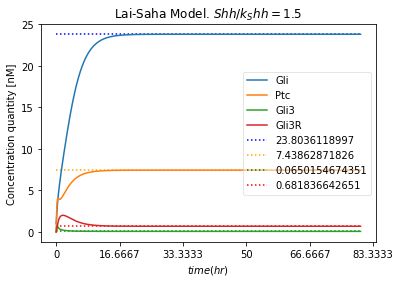
\includegraphics[width=0.8\textwidth]{lai1}
			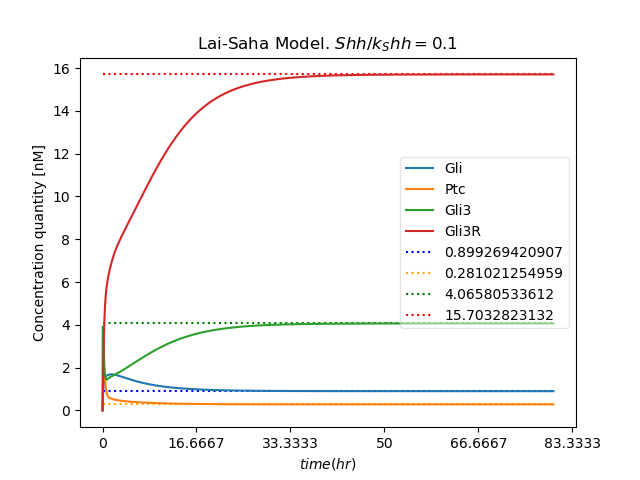
\includegraphics[width=0.8\textwidth]{lai2}
		\end{figure}
	\end{column}
	\begin{column}{0.5\textwidth}
		Bifurcaciones:
		\begin{figure}
			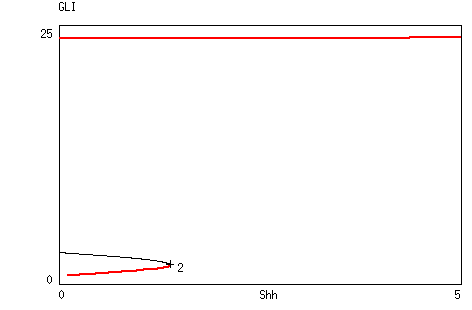
\includegraphics[width=0.9\textwidth]{diagramaweno1}
			
			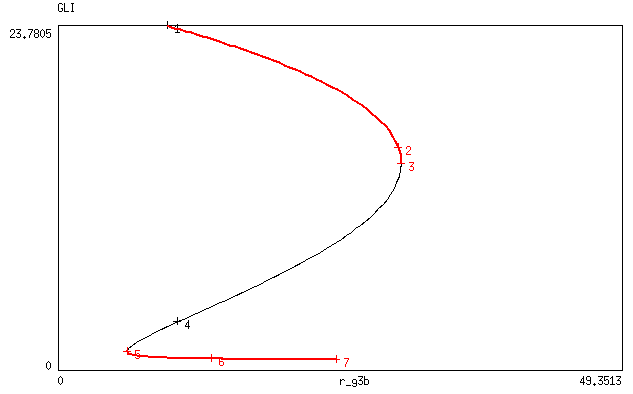
\includegraphics[width=0.9\textwidth]{gliVSr_g3b}
		\end{figure}
	\end{column}
\end{columns}
\end{frame}

\section{Modelo nuevo}

\subsection{Definición del modelo}

\begin{frame}
\frametitle{Nuevo Modelo (Enfoque Cambón-Sánchez 2017)}
\begin{columns}
	\begin{column}{0.5\textwidth}
		Claves:
		\begin{itemize}
			\item Proteólisis de $Gli_3$ según señalización de Shh y activación de la red.
		\end{itemize}
		Claves \color{red} BEWARE:
		\begin{itemize}
			\item Enfoque \textit{recruitment}.
			\item Expresión génica proporcional a la probabiliadd de unión de ARNp.
		\end{itemize}
	\end{column}
	\begin{column}{0.5\textwidth}
		{\tiny\[ \frac{dGli}{dt} = \color{red}{newBEWARE}\color{black}-k_{deg}Gli \]}
		{\tiny\[ \frac{dGli_3}{dt} = \frac{r_{g3b}}{Ptc}-Gli_3\left(k_{deg}+\frac{k_{g3rc}}{K_{g3rc}+Signal}\right), \]}
		{\tiny\[ \frac{dGli3R}{dt}= Gli_3\left(\frac{k_{g3rc}}{K_{g3rc}+Signal}\right)-k_{deg}Gli3R, \]}
		{\tiny\[ \frac{dPtc}{dt} = \color{red}c_bnewBEWARE\color{black}-k_{degp}Ptc.\]}
		
	\end{column}
\end{columns}
\end{frame}


\subsection{Resultados}

\begin{frame}
\frametitle{Modelo nuevo (Enfoque Cambón-Sánchez 2017)}
\begin{columns}
	\begin{column}{0.5\textwidth}
		Evolución temporal.
		\begin{figure}
			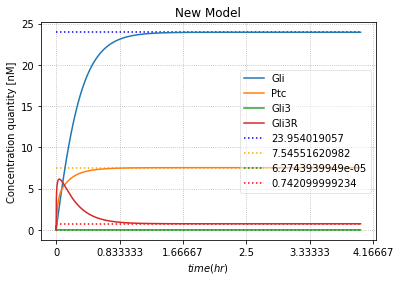
\includegraphics[width=1.1\textwidth]{new_beware_global}
		\end{figure}
	\end{column}
	\begin{column}{0.5\textwidth}
		Búsqueda de ceros.
		\begin{figure}
			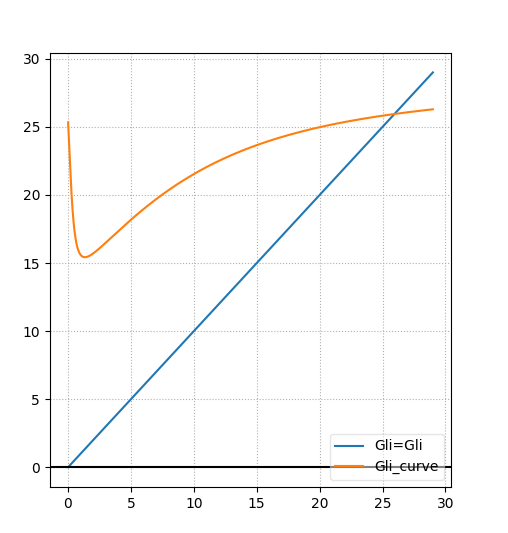
\includegraphics[width=0.9\textwidth]{zerosnew}
		\end{figure}
	\end{column}
\end{columns}
\end{frame}

\section{Conclusiones y futuro trabajo}

\begin{frame}
	\frametitle{Conclusiones y futuro trabajo}
	
	\begin{itemize}
		\item Problema de gran complejidad.
		\item Nuevos comportamientos descritos.
		\item Elaboración del modelo. 
		\item Motivar la profundización teórica.
		\item Orientar la investigación actual sentando un marco de referencia.
	\end{itemize}
\nocite{schaffer,cambon1, saha}
\end{frame}



\begin{frame}{References}
\small{Códigos, datos, latex, pdf: \url{https://github.com/thebooort/shh-signal-model}}
\bibliographystyle{ieeetr}
\bibliography{/data/Documentos/Universidad/Fisymat2018/TFM/shh-signal-model/bibliography/bibliografia}
\end{frame}



\end{document}